\documentclass{article}
\usepackage{tikz}
\usetikzlibrary{automata,positioning}
\begin{document}

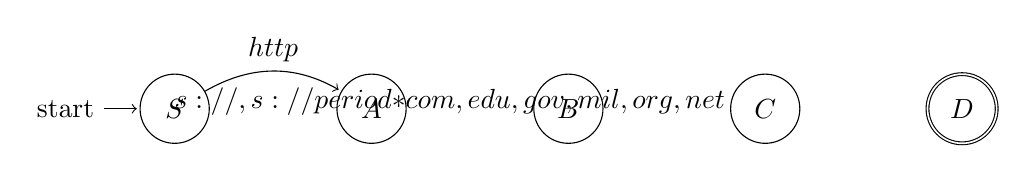
\begin{tikzpicture}[shorten >=1pt,node distance=2.5cm,on grid,auto]
  % Define states
  \node[state,initial] (S) {$S$};
  \node[state] (A) [right=of S] {$A$};
  \node[state] (B) [right=of A] {$B$};
  \node[state] (C) [right=of B] {$C$};
  \node [state, accepting] (D) [right=of C] {$D$};
  % Transitions
  \path[->]

    (S)  edge[bend left]  node {$http$} (A);
    (A) edge[bend right] node {$s://, s://$} (B);
    (B) edge[bend right] node {$period$} (C);
	(B) edge[loop above] node {$*$} ();
	(C) edge[bend right] node {$com, edu, gov, mil, org, net$} (D);
\end{tikzpicture}

\end{document}
